
\hypertarget{cv:registrarAccion}{\section{Registrar Acción}} \label{sec:registrarAccion}

	Esta funcionalidad le permitirá registrar una acción que perteneciente a una pantalla dentro del proyecto que se esta operando. 

		\subsection{Procedimiento}

			%Pasos de procedimiento
			\begin{enumerate}
	
			\item Oprima el botón \IURegistrar{} de la pantalla \ref{fig:GestionarAcciones} ''Gestionar Acciones''.
			
			\item Se mostrará la pantalla \ref{fig:registrarAccion} ''Registrar Acción''.

			%Pantalla
			\begin{figure}[H]
				\begin{center}
					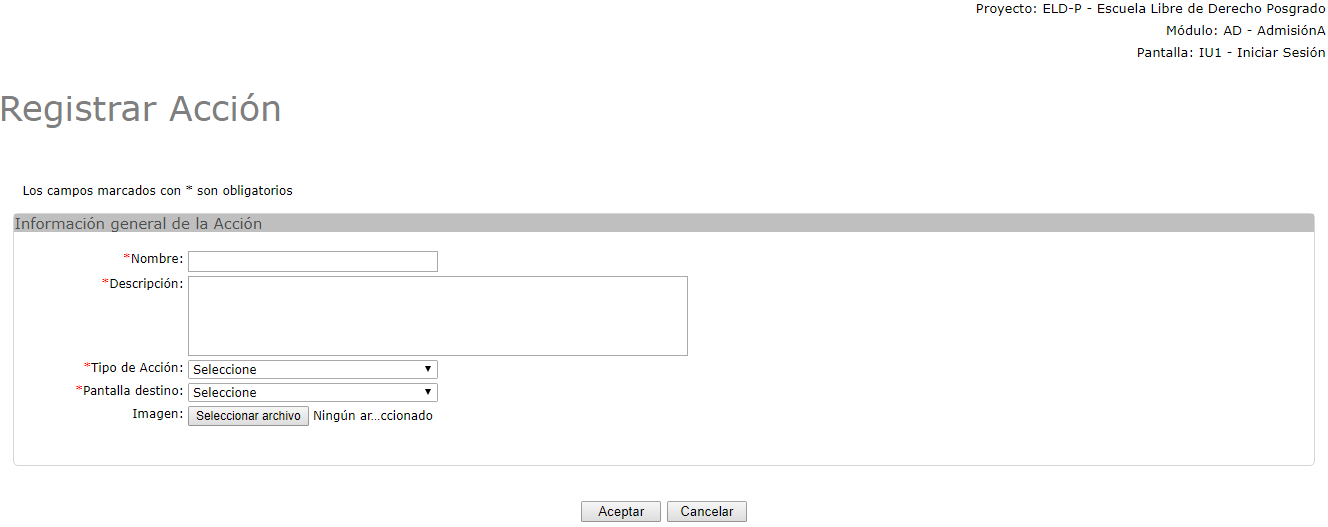
\includegraphics[scale=0.5]{roles/lider/pantallas/acciones/pantallas/IU11-1-1-1registrarAccion}
					\caption{Registrar Acción}
					\label{fig:registrarAccion}
				\end{center}
			\end{figure}
		
			\item Ingrese el nombre, una pequeña descripción, el tipo de acción a la que corresponde la acción y finalmente seleccione la pantalla destino que se mostrará cuando la acción se ejecute.
			
			\item Adjunte la imagen correspondiente, esta debe pesar como máximo 2 mb y tiene que ser en formato PNG.
			
			\item Oprima el botón \IUAceptar.
			
			\item Se mostrará el mensaje \ref{fig:accionRegistrada} en la pantalla \ref{fig:GestionarAcciones} ''Gestionar Acciones''.
			
			\begin{figure}[htbp!]
				\begin{center}
					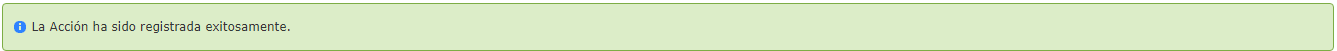
\includegraphics[scale=0.5]{roles/lider/pantallas/acciones/pantallas/IU11-1-1-1MSG1}
					\caption{MSG: Acción Registrada}
					\label{fig:accionRegistrada}
				\end{center}
			\end{figure}
			\end{enumerate}